\documentclass[tikz,border=3pt]{standalone}
\usepackage[T1]{fontenc}
\usepackage{times}
\usepackage{xcolor}
\usepackage{tikz}
\usetikzlibrary{arrows.meta,positioning,fit,shapes.geometric}

\definecolor{huntrixblue}{HTML}{1F5A7A}
\definecolor{huntrixteal}{HTML}{2A8C82}
\definecolor{huntrixgold}{HTML}{D59B32}
\definecolor{huntrixred}{HTML}{B5483A}
\definecolor{huntrixgray}{HTML}{EEF2F4}
\newcommand{\code}[1]{\texttt{#1}}

\begin{document}
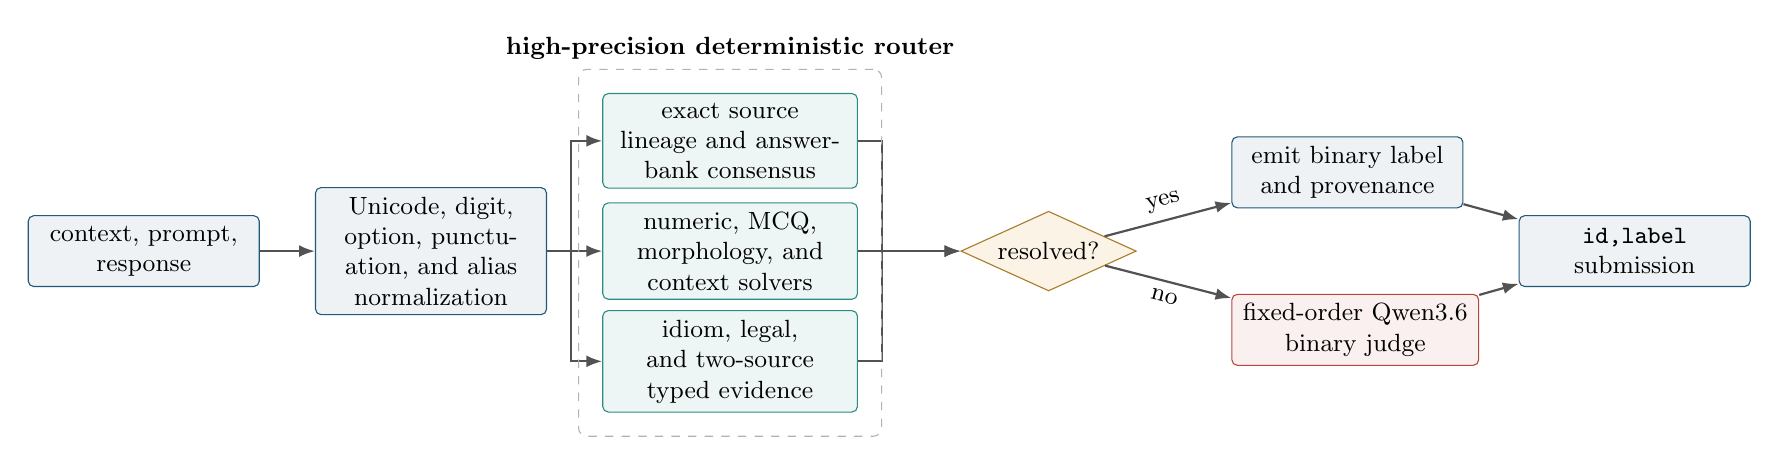
\begin{tikzpicture}[
  node distance=5.5mm and 7mm,
  every node/.style={font=\small},
  stage/.style={draw=huntrixblue, rounded corners=2pt, fill=huntrixgray,
                minimum height=9mm, align=center, text width=27mm},
  evidence/.style={draw=huntrixteal, rounded corners=2pt, fill=huntrixteal!8,
                   minimum height=9mm, align=center, text width=30mm},
  decision/.style={diamond, draw=huntrixgold!80!black, fill=huntrixgold!12,
                   aspect=2.2, align=center, inner sep=2pt},
  judge/.style={draw=huntrixred, rounded corners=2pt, fill=huntrixred!8,
                minimum height=9mm, align=center, text width=29mm},
  arrow/.style={-{Latex[length=2mm]}, thick, draw=black!68}
]
\node[stage] (input) {context, prompt, response};
\node[stage, right=of input] (norm) {Unicode, digit, option, punctuation, and alias normalization};
\node[evidence, right=of norm, yshift=14mm] (lineage) {exact source lineage and answer-bank consensus};
\node[evidence, right=of norm] (structured) {numeric, MCQ, morphology, and context solvers};
\node[evidence, right=of norm, yshift=-14mm] (typed) {idiom, legal, and two-source typed evidence};
\node[decision, right=13mm of structured] (resolved) {resolved?};
\node[stage, right=12mm of resolved, yshift=10mm] (emit) {emit binary label and provenance};
\node[judge, right=12mm of resolved, yshift=-10mm] (llm) {fixed-order Qwen3.6 binary judge};
\node[stage, right=of emit, yshift=-10mm] (csv) {\code{id,label} submission};

\draw[arrow] (input) -- (norm);
\draw[arrow] (norm.east) -- ++(3mm,0) |- (lineage.west);
\draw[arrow] (norm) -- (structured);
\draw[arrow] (norm.east) -- ++(3mm,0) |- (typed.west);
\draw[arrow] (lineage.east) -- ++(3mm,0) |- (resolved.west);
\draw[arrow] (structured) -- (resolved);
\draw[arrow] (typed.east) -- ++(3mm,0) |- (resolved.west);
\draw[arrow] (resolved) -- node[above,sloped]{yes} (emit);
\draw[arrow] (resolved) -- node[below,sloped]{no} (llm);
\draw[arrow] (emit) -- (csv);
\draw[arrow] (llm) -- (csv);

\node[draw=black!30, dashed, rounded corners=3pt, fit=(lineage)(structured)(typed),
      label={[font=\small\bfseries]above:high-precision deterministic router},
      inner sep=3mm] {};
\end{tikzpicture}
\end{document}
